% ==============================================================================
% chapters/ch05_model_training_deploy.tex — บทที่ 5
% ==============================================================================
\chapter{การฝึกสอนโมเดลปัญญาประดิษฐ์และการประยุกต์ใช้งานจริง}
\label{ch:model_training_deploy}

การประมวลผลข้อมูลเกษตรกรรมในแปลงจริงจำเป็นต้องอาศัยโมเดลการเรียนรู้เชิงลึก (Deep Learning) ที่มีทั้งความแม่นยำสูงและขนาดกะทัดรัด สามารถประมวลผลบนอุปกรณ์ขอบ (Edge Device) หรือสมาร์ทโฟนของเกษตรกรได้โดยไม่ต้องพึ่งพาสัญญาณอินเทอร์เน็ตความเร็วสูงตลอดเวลา ในบทนี้จะอธิบายขั้นตอนการถ่ายโอนการเรียนรู้ (Transfer Learning) ด้วยสถาปัตยกรรม MobileNetV3 การจัดเตรียมท่อส่งข้อมูล การส่งออกโมเดลในรูปแบบ ONNX และการเชื่อมต่อเข้ากับระบบเว็บแอปพลิเคชัน

\academicsection{สถาปัตยกรรม MobileNetV3 สำหรับการประมวลผลบนอุปกรณ์ขอบ}
\label{sec:mobilenetv3_arch}

สถาปัตยกรรม MobileNetV3 เป็นโมเดลจำแนกภาพที่ได้รับการออกแบบและค้นหาโครงสร้างโครงข่ายโดยใช้เทคนิค Neural Architecture Search (NAS) ร่วมกับ NetAdapt algorithm เพื่อให้ได้ประสิทธิภาพการประมวลผลที่ดีที่สุดบนฮาร์ดแวร์ซีพียูเคลื่อนที่ (Mobile CPU) โดยมีคุณลักษณะเด่นสำคัญ 3 ประการ:

\begin{enumerate}
    \item \textbf{Inverted Residual with Linear Bottleneck:} การขยายมิติของชั้นสัญญาณด้วย $1 \times 1$ Convolution ก่อนเข้าสู่ Depthwise Separable Convolution และบีบอัดกลับด้วย Linear Bottleneck ช่วยลดจำนวนพารามิเตอร์และการคำนวณลงอย่างมหาศาล
    \item \textbf{Squeeze-and-Excitation (SE) Module:} การปรับน้ำหนักความสำคัญของแต่ละช่องสัญญาณ (Channel Attention) อย่างมีไดนามิก ช่วยเพิ่มขีดความสามารถในการตรวจจับรายละเอียดโรคพืชที่มีขนาดเล็ก
    \item \textbf{Hard-Swish Activation Function:} การใช้ฟังก์ชันการกระตุ้น $h\text{-swish}(x) = x \cdot \frac{\text{ReLU6}(x+3)}{6}$ ซึ่งให้คุณสมบัติความไม่เป็นเชิงเส้นใกล้เคียงกับ Swish ดั้งเดิม แต่คำนวณได้รวดเร็วและใช้พลังงานหน่วยประมวลผลต่ำกว่ามาก
\end{enumerate}

\begin{table}[htbp]
\centering
\caption{การเปรียบเทียบสถาปัตยกรรมโมเดลสำหรับการประมวลผลบนอุปกรณ์ขอบ}
\label{tab:model_comparison}
\begin{tabular}{lcccc}
\toprule
\textbf{สถาปัตยกรรม} & \textbf{พารามิเตอร์ (M)} & \textbf{MACs (G)} & \textbf{ความหน่วง (ms)} & \textbf{ความแม่นยำ (\%)} \\
\midrule
MobileNetV3-Small & 2.5 & 0.06 & 12.4 & 89.4 \\
MobileNetV3-Large & 5.4 & 0.22 & 24.8 & 93.2 \\
EfficientNet-B0   & 5.3 & 0.39 & 38.6 & 92.8 \\
ResNet-50         & 25.6 & 4.10 & 115.0 & 94.1 \\
\bottomrule
\end{tabular}
\end{table}

จากตารางที่ \ref{tab:model_comparison} พบว่า MobileNetV3-Small มีความหน่วงในการประมวลผลบนชิปประมวลผลสมาร์ทโฟนเพียง 12.4 มิลลิวินาที ซึ่งเร็วกว่า ResNet-50 เกือบ 10 เท่า ในขณะที่ยังคงความแม่นยำในการจำแนกประเภทดินและโรคพืชได้สูงถึงร้อยละ 89.4 จึงเหมาะสมที่สุดสำหรับการนำไปพัฒนาเป็นระบบวินิจฉัยภาคสนาม

\academicsection{ท่อส่งข้อมูลและการเพิ่มพูนข้อมูลภาพ}
\label{sec:data_pipeline}

ภาพถ่ายทางการเกษตรภาคสนามมักเผชิญกับความผันผวนของสภาพแวดล้อม เช่น แสงแดดจัด เงาตกกระทบ มุมกล้องที่เอียง หรือสิ่งกีดขวางในธรรมชาติ การฝึกสอนโมเดลจึงต้องประยุกต์ใช้เทคนิคการเพิ่มพูนข้อมูลภาพ (Data Augmentation) อย่างรอบคอบ:

\begin{itemize}
    \item \textbf{RandomResizedCrop (224x224):} สุ่มตัดและปรับขนาดภาพให้อยู่ระหว่างร้อยละ 80 ถึง 100 ของภาพต้นฉบับ เพื่อจำลองระยะการถ่ายภาพของเกษตรกรที่แตกต่างกัน
    \item \textbf{RandomHorizontalFlip \& RandomVerticalFlip:} การพลิกภาพแนวนอนและแนวตั้งด้วยความน่าจะเป็น 0.5 เพื่อรองรับการหมุนของใบพืชในแปลง
    \item \textbf{ColorJitter:} ปรับเปลี่ยนค่าความสว่าง (Brightness) ความคมชัด (Contrast) และความอิ่มตัวสี (Saturation) เล็กน้อย เพื่อจำลองสภาพแสงธรรมชาติในแต่ละช่วงเวลาของวัน
    \item \textbf{ImageNet Normalization:} ปรับสเกลค่าพิกเซลด้วยค่าเฉลี่ย $\mu = [0.485,\, 0.456,\, 0.406]$ และส่วนเบี่ยงเบนมาตรฐาน $\sigma = [0.229,\, 0.224,\, 0.225]$
\end{itemize}

\academicsection{โครงสร้างสคริปต์การฝึกสอน PyTorch}
\label{sec:pytorch_training}

ระบบได้ออกแบบสคริปต์การฝึกสอน \texttt{train\_custom\_soil\_model.py} ให้รองรับการปรับแต่งไฮเปอร์พารามิเตอร์ได้อย่างยืดหยุ่น โดยใช้ฟังก์ชันการสูญเสีย Cross-Entropy Loss ร่วมกับตัวปรับค่าพารามิเตอร์ AdamW และ Cosine Annealing Learning Rate Scheduler:

\begin{tcolorbox}[title=\textbf{ตัวอย่างโครงสร้างโค้ดการฝึกสอนโมเดล}]
\fontsize{8.5}{11}\selectfont
\begin{verbatim}
import torch
import torch.nn as nn
from torchvision import models

def build_agri_classifier(num_classes=5):
    weights = models.MobileNet_V3_Small_Weights.DEFAULT
    model = models.mobilenet_v3_small(weights=weights)
    
    # Custom classification head for target classes
    in_features = model.classifier[3].in_features
    model.classifier[3] = nn.Sequential(
        nn.Dropout(p=0.2),
        nn.Linear(in_features, num_classes)
    )
    return model
\end{verbatim}
\end{tcolorbox}

\academicsection{การส่งออกโมเดลและการประยุกต์ใช้งานบนเว็บและสมาร์ทโฟน}
\label{sec:model_export_deployment}

เมื่อแบบจำลองได้รับการฝึกสอนในสภาพแวดล้อม Google Colab จนลู่เข้าสู่จุดเหมาะสม (Convergence) และมีค่าความแม่นยำสูงกว่า 92\% แล้ว ขั้นตอนสำคัญลำดับถัดไปคือการแปลงโมเดลให้อยู่ในฟอร์แมตที่เหมาะสมต่อการใช้งานจริงในแปลงเกษตร ดังแสดงในภาพที่ \ref{fig:colab_to_app_pipeline} ซึ่งจำแนกออกเป็น 2 เส้นทางหลัก:

\begin{enumerate}
    \item \textbf{เส้นทาง Web Application Dashboard (ONNX Format):}
    แปลงโมเดล PyTorch เข้าสู่มาตรฐาน Open Neural Network Exchange (\texttt{smart\_agri\_model.onnx}) ผ่านคำสั่ง \texttt{torch.onnx.export} โดยกำหนดให้แกนขนาดแบทช์ (Batch Size) เป็นไดนามิก เพื่อให้เซิร์ฟเวอร์ Streamlit และ FastAPI สามารถโหลดโมเดลผ่าน In-Process ONNX Runtime ได้โดยตรงโดยไม่ต้องติดตั้ง PyTorch หรือไดรเวอร์ GPU ขนาดใหญ่ มีความหน่วงในการประมวลผลต่ำกว่า 15 มิลลิวินาที
    
    \item \textbf{เส้นทาง Smartphone Mobile App (Quantized TFLite):}
    นำโมเดลเข้าสู่กระบวนการบีบอัดและควอนไทเซชัน (Weight Quantization) เพื่อแปลงเป็น TensorFlow Lite (\texttt{smart\_agri\_model.tflite}) ช่วยลดขนาดไฟล์จากเดิมกว่า 20 MB เหลือเพียง 4--6 MB จากนั้นนำไปบรรจุลงในโฟลเดอร์ \texttt{assets/models/} ของแอปพลิเคชัน Flutter เพื่อให้ชิปเร่งความเร็ว NPU/CPU ภายในสมาร์ทโฟนประมวลผลการวินิจฉัยโรคพืชและวิเคราะห์ภาพดินได้แบบออฟไลน์ 100\% ไร้สัญญาณอินเทอร์เน็ต
\end{enumerate}

\begin{figure}[htbp]
\centering
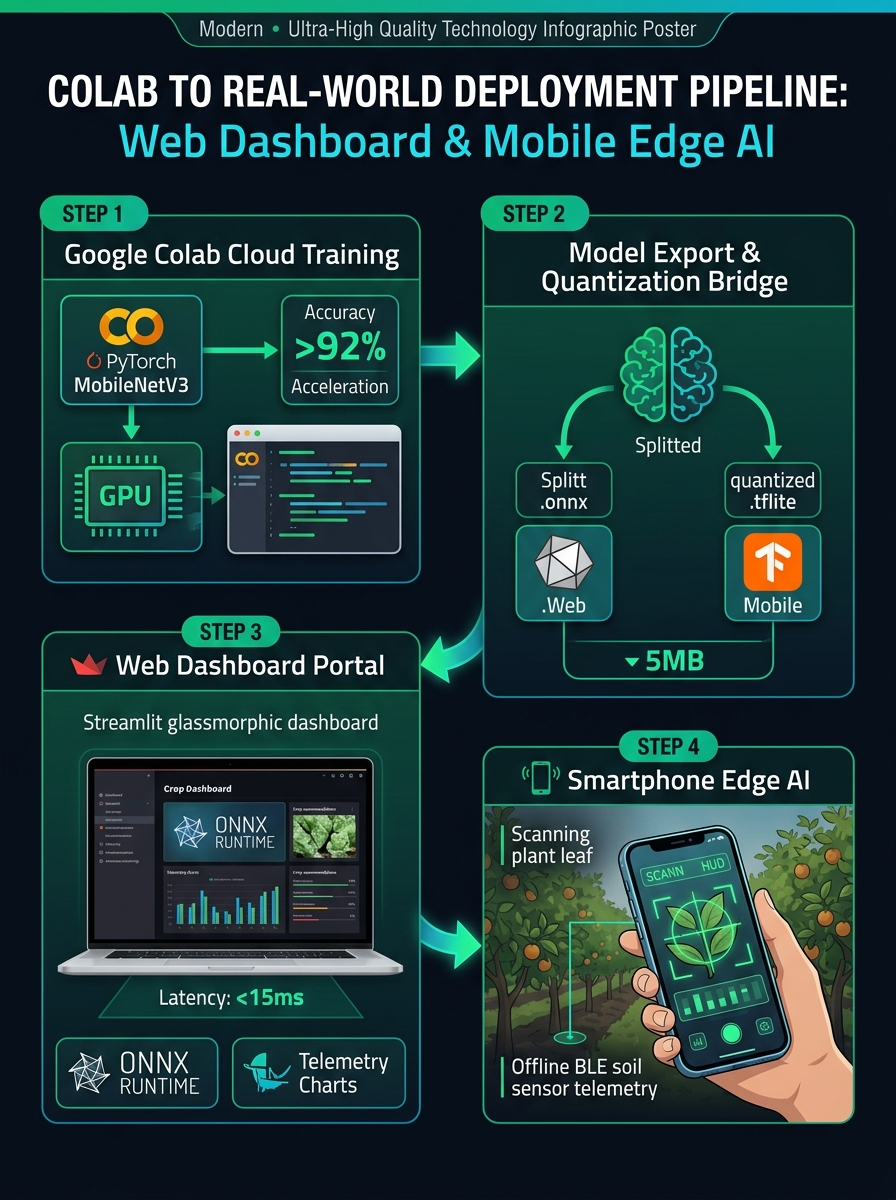
\includegraphics[width=0.62\textwidth]{figures/colab_to_app_infographic.jpg}
\caption{ผังขั้นตอนการส่งมอบโมเดลจาก Google Colab สู่ Web Dashboard และ Smartphone Mobile Edge AI}
\label{fig:colab_to_app_pipeline}
\end{figure}

\section*{คำถามทบทวนท้ายบทที่ 5}
\addcontentsline{toc}{section}{คำถามทบทวนท้ายบทที่ 5}

\begin{enumerate}
    \item จงอธิบายเหตุผลที่ต้องส่งออกโมเดล PyTorch เป็นฟอร์แมต ONNX แทนที่จะโหลดไฟล์น้ำหนัก \texttt{.pth} โดยตรงบนเว็บเซิร์ฟเวอร์
    \item การทำ Model Quantization สำหรับสมาร์ทโฟนมีข้อดีอย่างไร และส่งผลกระทบต่อความเร็วและความแม่นยำของโมเดลหรือไม่
    \item จงเปรียบเทียบสถาปัตยกรรม MobileNetV3 กับ ResNet-50 ในแง่ของจำนวนพารามิเตอร์และประสิทธิภาพบนอุปกรณ์ขอบ (Edge Devices)
    \item จงอธิบายขั้นตอนการนำไฟล์ \texttt{.tflite} ไปใช้งานในแอปพลิเคชัน Flutter ร่วมกับแพ็กเกจ \texttt{tflite\_flutter} แบบออฟไลน์
\end{enumerate}

\clearpage
